\documentclass{standalone}
\usepackage{tikz}
\begin{document}
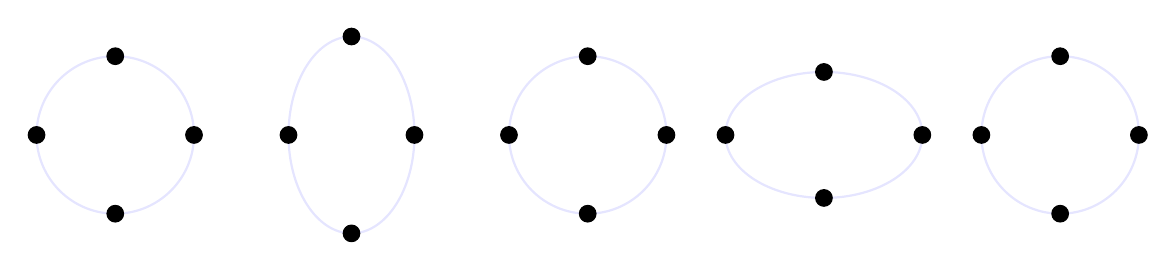
\begin{tikzpicture}
    \draw[color=blue!10, thick](0,0) circle (1);
    \filldraw[black] ( 0, 1) circle (3pt);
    \filldraw[black] ( 0,-1) circle (3pt);
    \filldraw[black] ( 1, 0) circle (3pt);
    \filldraw[black] (-1, 0) circle (3pt);
   
    \draw[color=blue!10, thick] (3,0) ellipse (0.8 and 1.25);
    \filldraw[black] (3,   1.25) circle (3pt);
    \filldraw[black] (3,  -1.25) circle (3pt);
    \filldraw[black] (3.8, 0)    circle (3pt);
    \filldraw[black] (2.2, 0)    circle (3pt);
   
    \draw[color=blue!10, thick](6,0) circle (1);
    \filldraw[black] ( 6, 1) circle (3pt);
    \filldraw[black] ( 6,-1) circle (3pt);
    \filldraw[black] ( 5, 0) circle (3pt);
    \filldraw[black] ( 7, 0) circle (3pt);
   
    \draw[color=blue!10, thick] (9,0) ellipse (1.25 and 0.8);
    \filldraw[black] (9,     0.8) circle (3pt);
    \filldraw[black] (9,    -0.8) circle (3pt);
    \filldraw[black] (7.75,  0)   circle (3pt);
    \filldraw[black] (10.25, 0)   circle (3pt);

    \draw[color=blue!10, thick](12,0) circle (1);
    \filldraw[black] (12, 1) circle (3pt);
    \filldraw[black] (12,-1) circle (3pt);
    \filldraw[black] (11, 0) circle (3pt);
    \filldraw[black] (13, 0) circle (3pt);
   
\end{tikzpicture}
\end{document}


